\chapter{Dlsgui}

\label{chap:dlsgui}
This chapter explains the installation of \texttt{dlsgui} which is the
newer viewer for DLS.

\section{Install prerequesites}

The following prerequesites must be installed to compile DLS.

\subsubsection{Binary packages}
\begin{verbatim}
sudo apt install  qt5-qmake qt5-default libqt5svg5-dev qttools5-dev

\end{verbatim}

\noindent Compile widgets

\begin{verbatim}
cd /tmp/dls/widgets
qmake
make
\end{verbatim}


\noindent Compile dlsgui
\begin{verbatim}
cd /tmp/dls/gui
qmake
make
\end{verbatim}

\noindent Install the program

\begin{verbatim}
sudo -i
cd /tmp/dls
install -m755 -oroot -groot gui/dlsgui /opt/etherlab/bin/
install -m644 -oroot -groot widgets/libDlsWidgets.so  /opt/etherlab/lib/
echo /opt/etherlab/lib > /etc/ld.so.conf.d/etherlab.conf
ldconfig
\end{verbatim}



\section{Run dlsgui}


\begin{verbatim}
/opt/etherlab/bin/dlsgui
\end{verbatim}

\noindent Open the datasource menu
\begin{center}
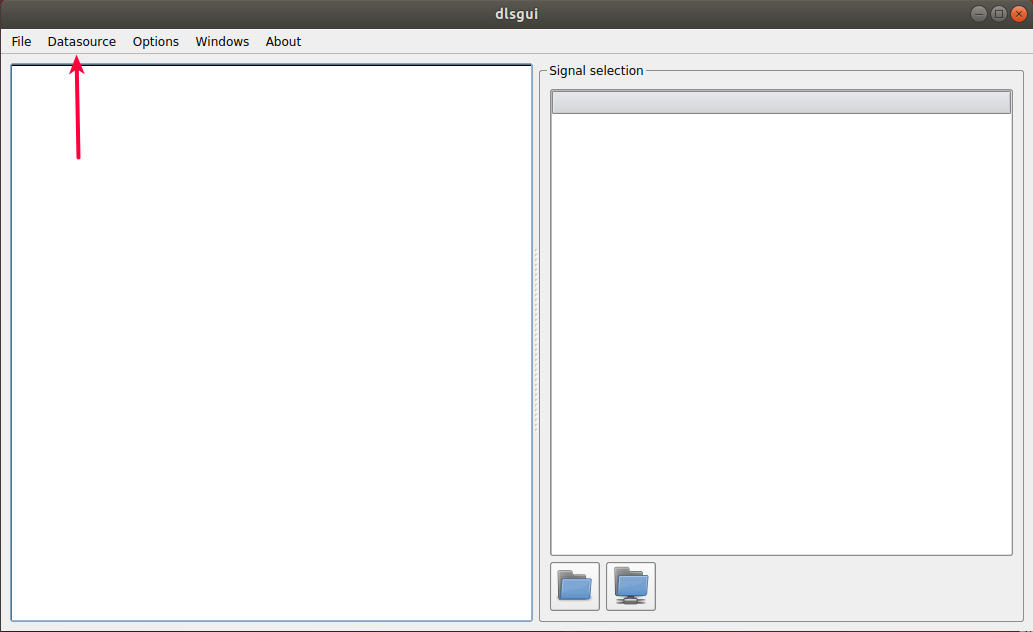
\includegraphics[width=0.9\textwidth]{genpicts/dlsgui-00.eps}
\end{center}

\noindent Then \textit{Add remote datasource...}
\begin{center}
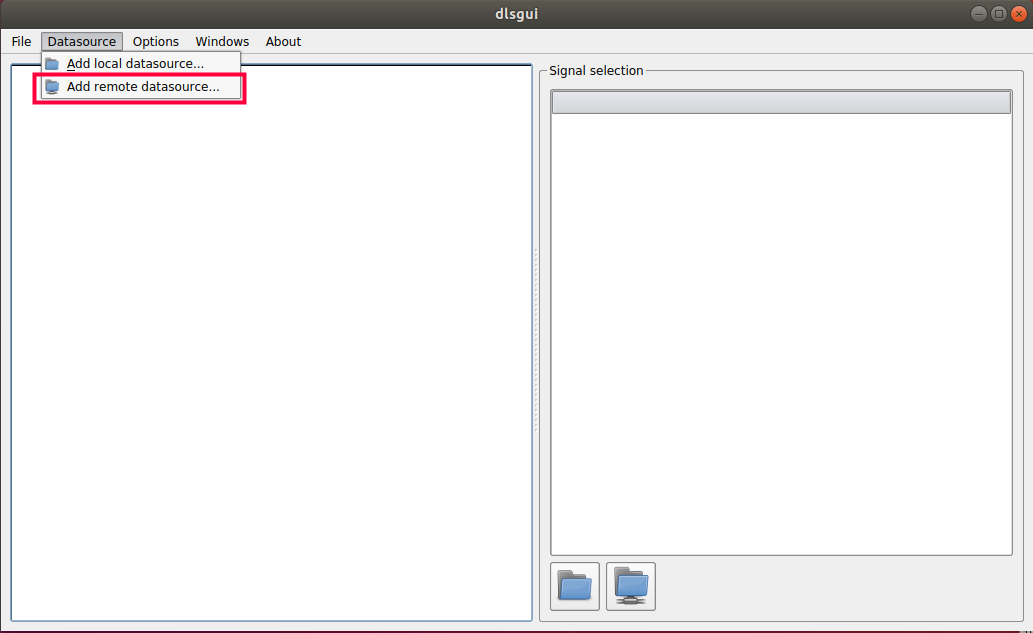
\includegraphics[width=0.9\textwidth]{genpicts/dlsgui-01.eps}
\end{center}

\noindent Fill the form
\begin{center}
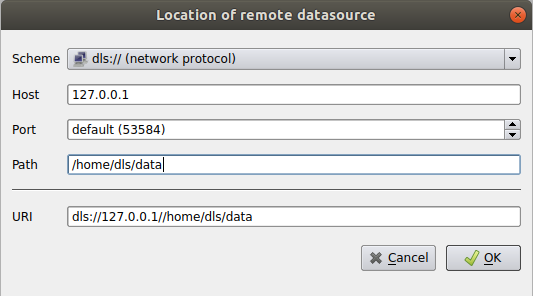
\includegraphics[width=0.9\textwidth]{genpicts/dlsgui-02.eps}
\end{center}


\noindent Expand the tree in the right panel to find
the channel to display, then drag-and-drop it to the left panel.
\begin{center}
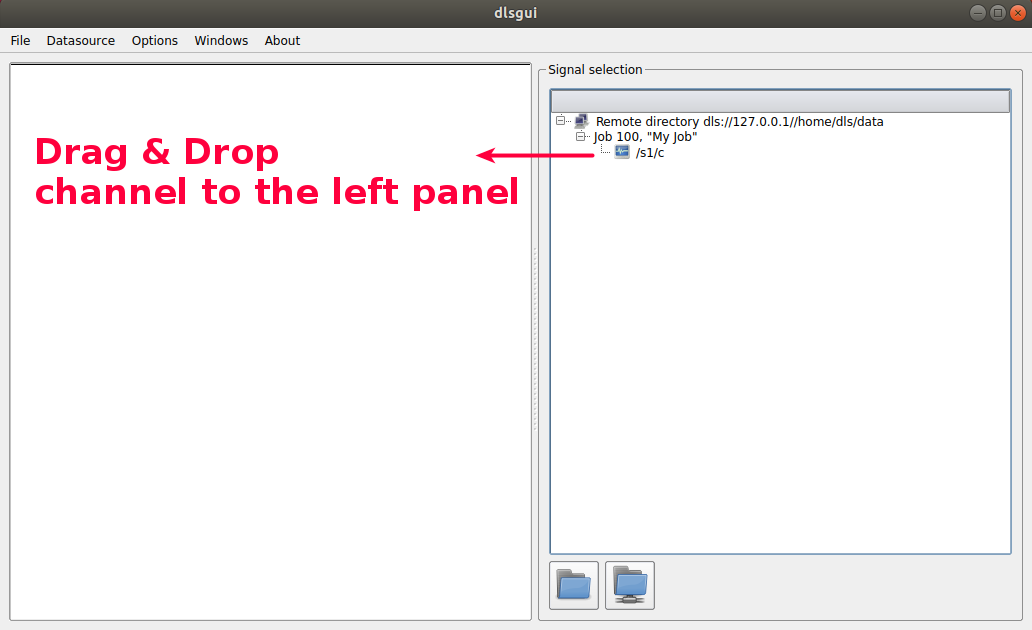
\includegraphics[width=0.9\textwidth]{genpicts/dlsgui-03.eps}
\end{center}

\noindent Zoom and navigate with keyboard and mouse inside the left panel
to see the information.
\begin{center}
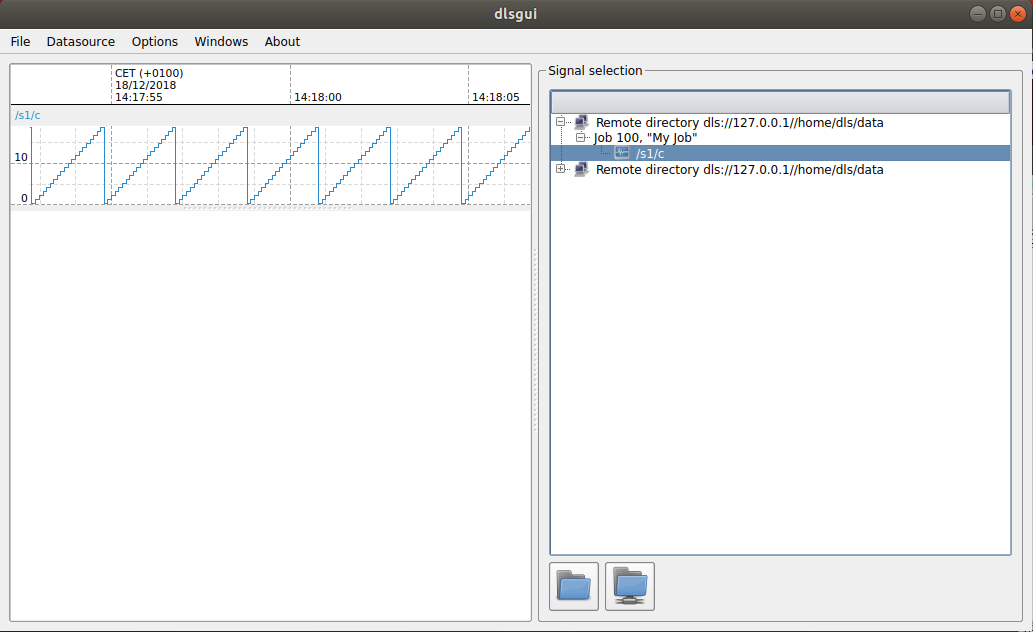
\includegraphics[width=0.9\textwidth]{genpicts/dlsgui-04.eps}
\end{center}
